\documentclass[border=4pt]{standalone}
\usepackage{tikz}
\usetikzlibrary{arrows,positioning}
\begin{document}
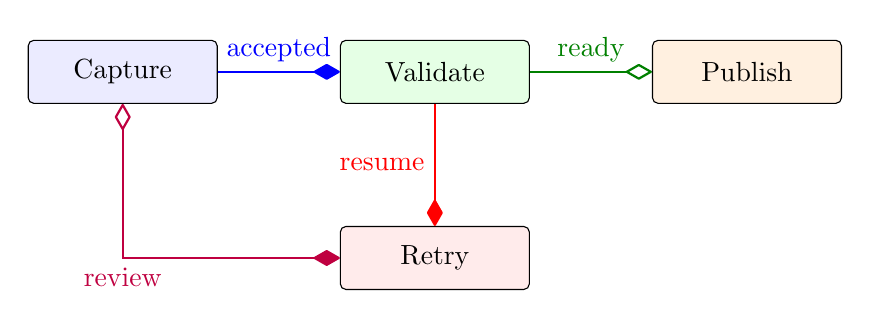
\begin{tikzpicture}[
  node distance=1.55cm,
  stage/.style={draw, rounded corners=2pt, minimum width=2.4cm, minimum height=8mm, align=center}
]
  \node[stage,fill=blue!8] (capture) {Capture};
  \node[stage,fill=green!10,right=of capture] (validate) {Validate};
  \node[stage,fill=orange!12,right=of validate] (publish) {Publish};
  \node[stage,fill=red!8,below=of validate] (retry) {Retry};

  \draw[blue,line width=.8pt,-diamond] (capture) -- node[above]{accepted} (validate);
  \draw[green!50!black,line width=.8pt,-{open diamond}] (validate) -- node[above]{ready} (publish);
  \draw[red,line width=.8pt,{diamond}-] (retry) -- node[left]{resume} (validate);
  \draw[purple,line width=.8pt,{open diamond}-{diamond}] (capture) |- node[below]{review} (retry);
\end{tikzpicture}
\end{document}
